\chapter{Methodology}
	The whole thesis research is divided into three stages. In the first stage, a 3D model with exact geometry and orientation for each building is built using \textit{DesignBuilder (version4.7)}, the building material and the thermal performance of the building envelopes are given by measurements in the previous research. In the second stage, the two buildings are subject to building energy analyses using both SIA 380/1 standard tool and EnergyPlus. The models are then verified and calibrated by comparing the measured historical indoor temperature with the calculated indoor temperature . In the final stage, a set of key building parameters are varied and stochastic building environment is subject to analyses using jE-Plus. Further analyses would find out the correlation between parameters as well as the influence about climate data.

	\section{Office Building Introduction}
		
		\begin{figure}[h!]
		\centering
		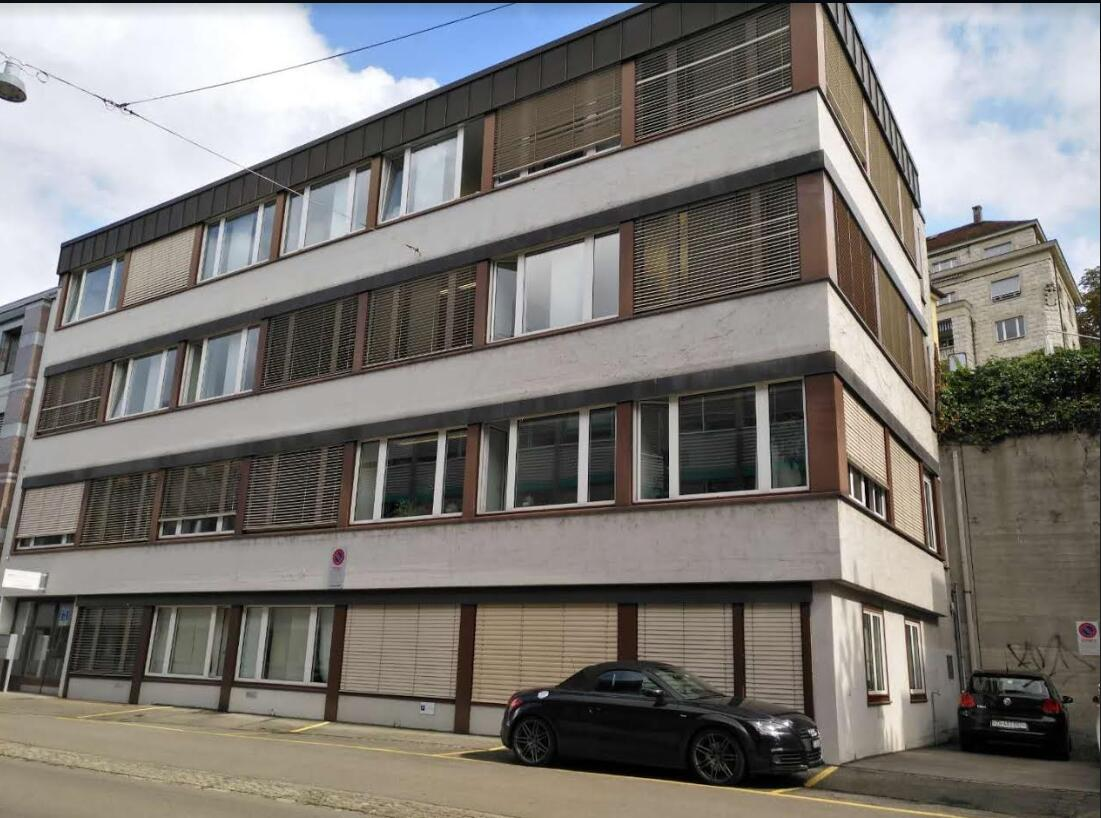
\includegraphics[scale=0.5]{Sumatra_photo.jpg}
		\caption{Sumatrastrasse 10 Office Building}
		\label{fig:Sumatra_photo}
		\end{figure}
		 
		
		According to the given information, the office building is constructed in 1951 and is located at Sumatrastrasse 10, 8006 Zurich, Switzerland. The building has 4 floors and a basement. The building  is facing west, and the window-to-wall ratio is 59\% on its west and south facade. The east facade of its ground floor and first floor is submerged into ground and there are heavy cover of plants on the upper floors with only a few necessary windows. There is also an underground floor used as warehouse and it's not included in any building model in this thesis.\\

		Figure \ref{fig:sumatra_og2} and \ref{fig:sumatra_og3} below are the floor plans of the building.
		The floor layout of ground floor, first floor and second floor are thought to be identical, and the third would have some small differences. For each floor, there is a toilet, a small office and 2 middle offices and a staircase. There is also a big office in each floor at the south side at ground floor, first floor and second floor. At the third floor, part of the big office and the corridor become a meeting room and a small pastry area as shown in the figures below. The detail building envelope material and modelling parameters are at chapter \textit{Methodology}.
		
		\begin{figure}[H]
		  \centering
		  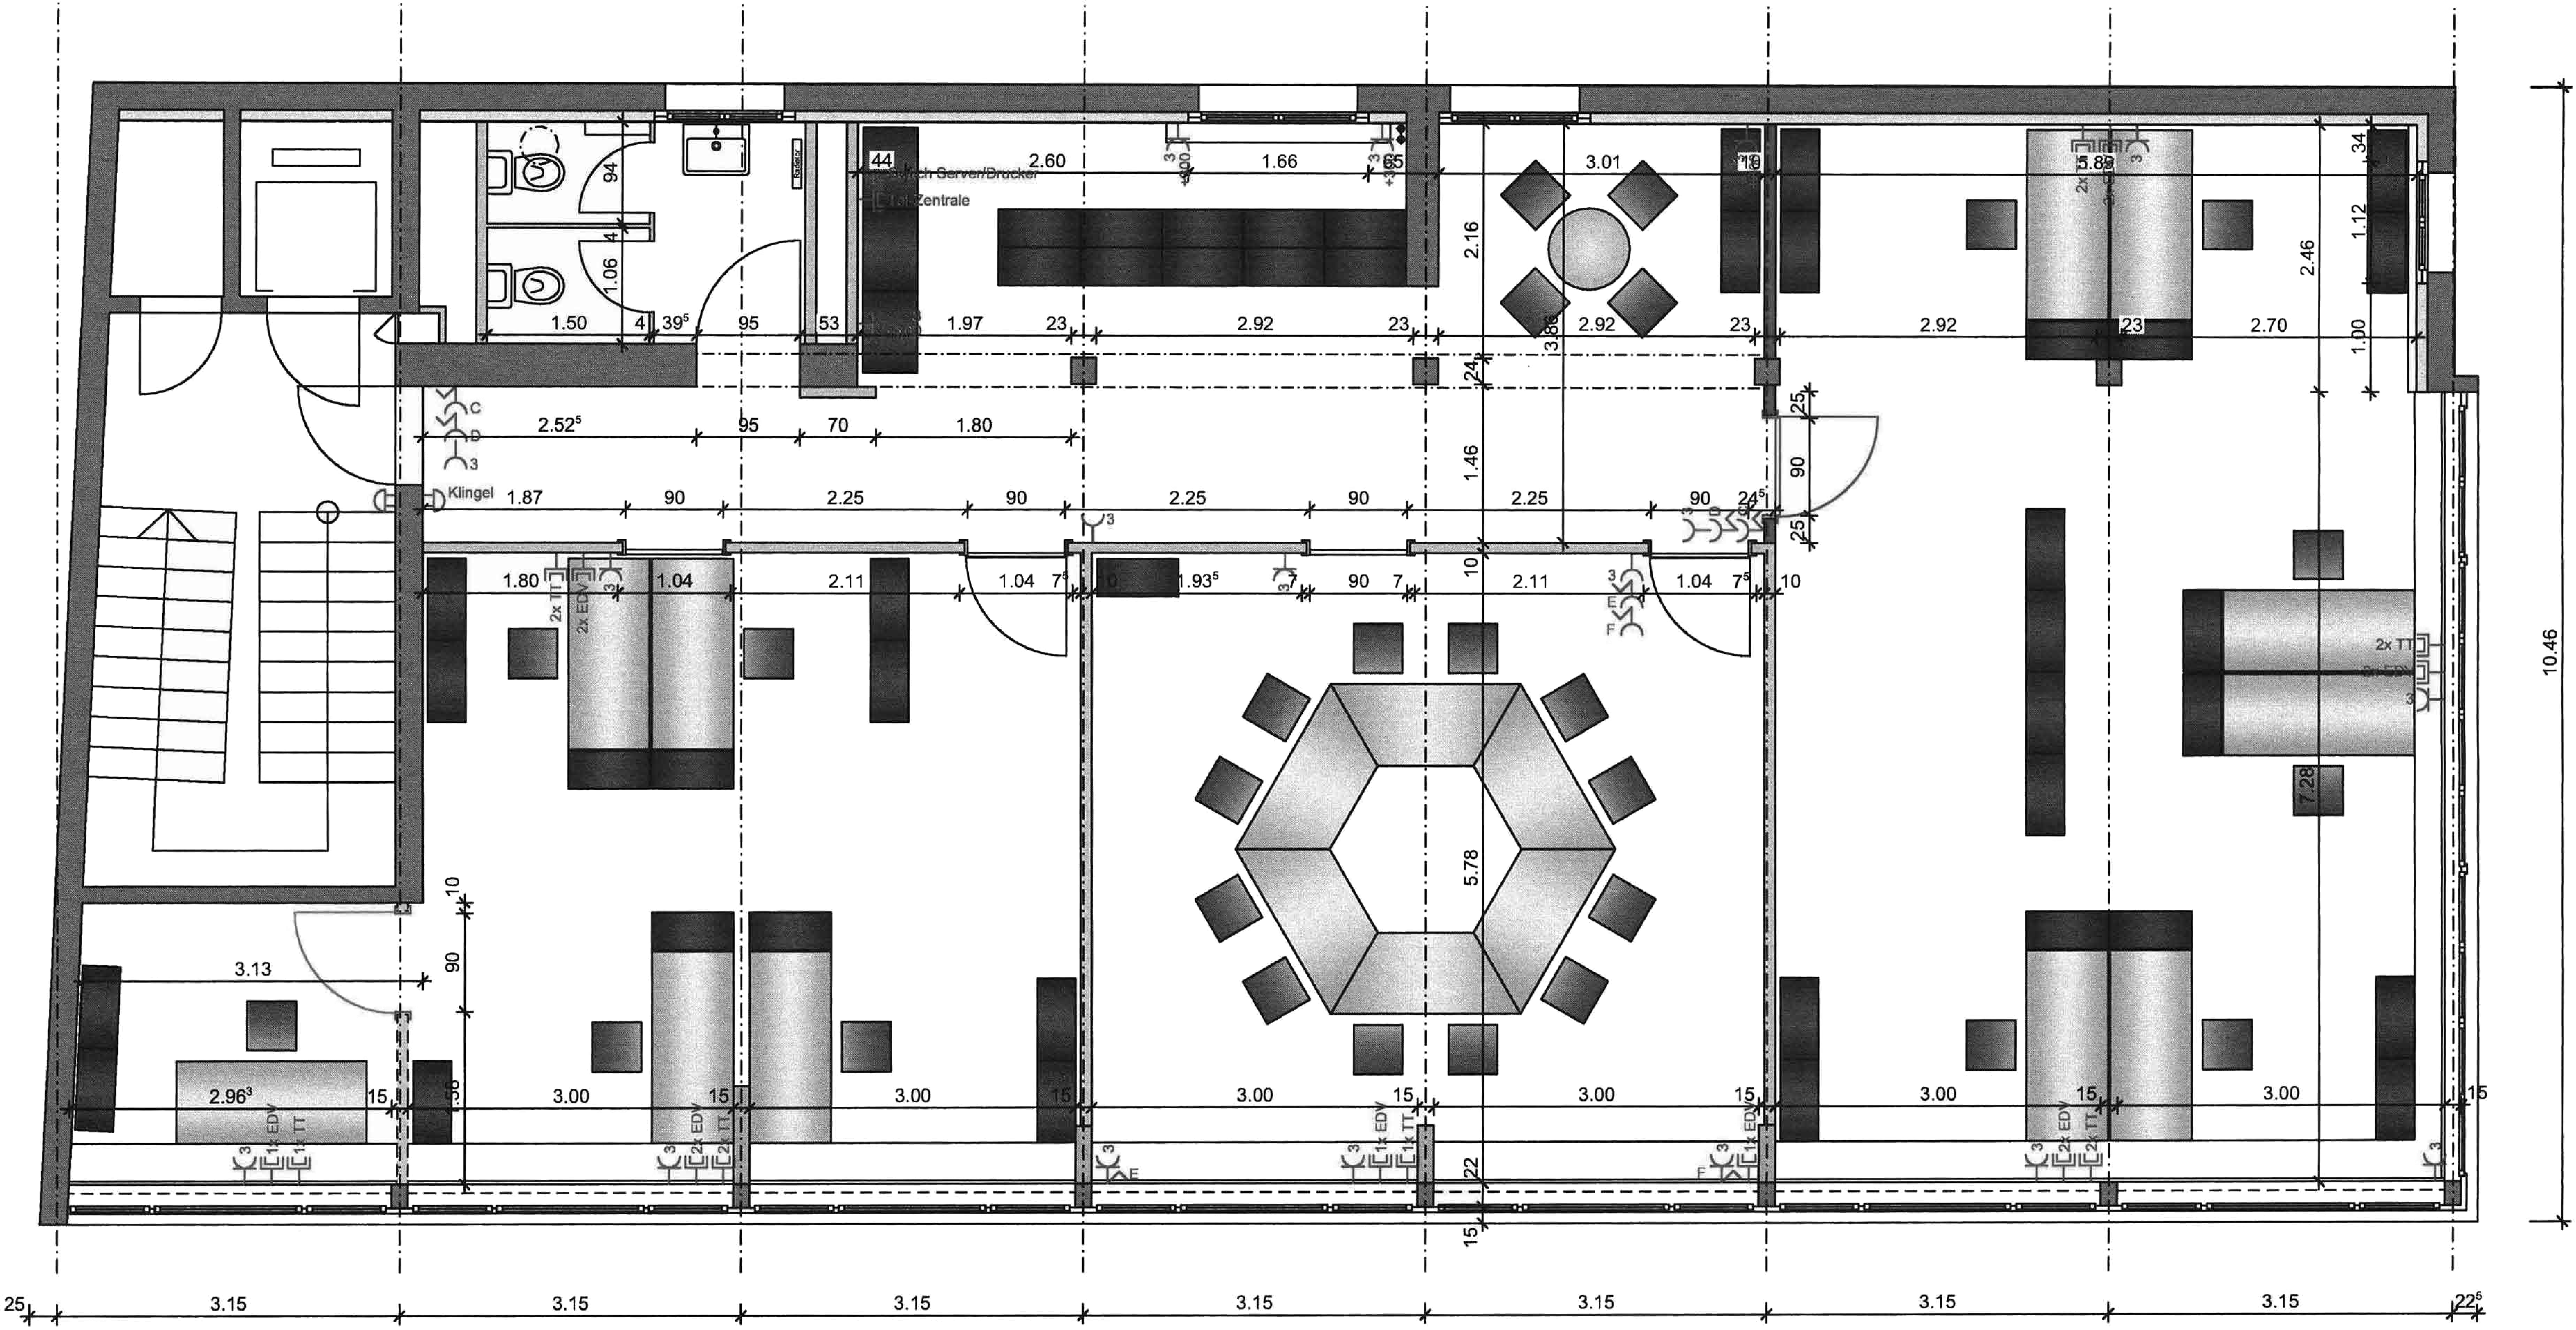
\includegraphics[scale=0.13]{Sumatra_OG2_Plan.pdf}
		  \caption{Floor plan of office building (Sumatra) ground floor to 2$^{nd}$ floor}
		  \label{fig:sumatra_og2}
		 \end{figure}

		\begin{figure}[H]
		  \centering
		  \includegraphics[scale=0.13]{Sumatra_OG3_Plan.pdf}
		  \caption{Floor plan of office building (Sumatra) 3$^{rd}$ floor}
		  \label{fig:sumatra_og3}
		\end{figure}
	
		
	\section{Residential Building Introduction}
		Figure \ref{fig:hongg_NE} and \ref{fig:hongg_SW} below show the photo of the residential building. The residential building is a part of a multi-family town house constructed in 1894. It is located at Honggerstrasse 23, 8037 Zurich, Switzerland. The building has 5 floors, the top floor is a loft and there is also an extra basement. There are 4 apartments in the building. The first apartment occupies the ground floor and the first floor, and the other 3 apartments each occupy one floor. Figure \ref{fig:hongg_eg_plan} and Figure \ref{fig:hongg_og1_plan} below are the floor plans of the residential building. The ground floor is connected with the first floor internally via a small staircase behide the kitchen. The black and red lines in Figure \ref{fig:hongg_eg_plan} show the ground floor layout and the yellow line indicates the layout of the upper floor. Similarily, Figure \ref{fig:hongg_og1_plan} shows the floor plans from first floor upward. The  red line indicates the layout of first floor and the yellow line shows the layout from second floor up. The detail building envelope material and modelling parameters are at chapter \textit{Methodology}.\\
		

		\begin{figure}[htbp]
		\centering
		\begin{minipage}[t]{0.48\textwidth}
		\centering
		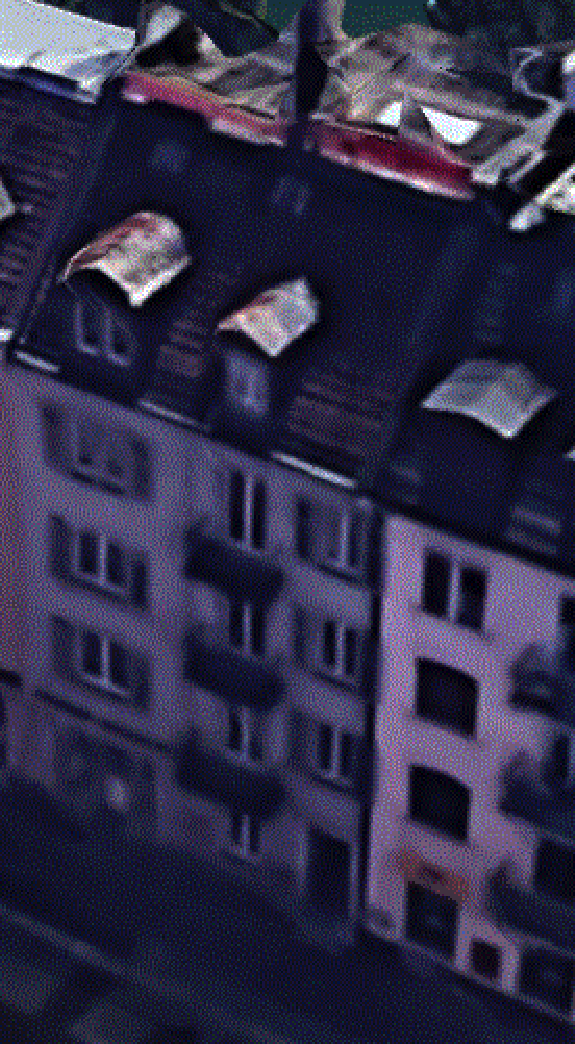
\includegraphics[width=5cm]{Hongg_photo1.pdf}
		\caption{Honggerstrasse 23, NE Side}
		\label{fig:hongg_NE}
		\end{minipage}
		\begin{minipage}[t]{0.48\textwidth}
		\centering
		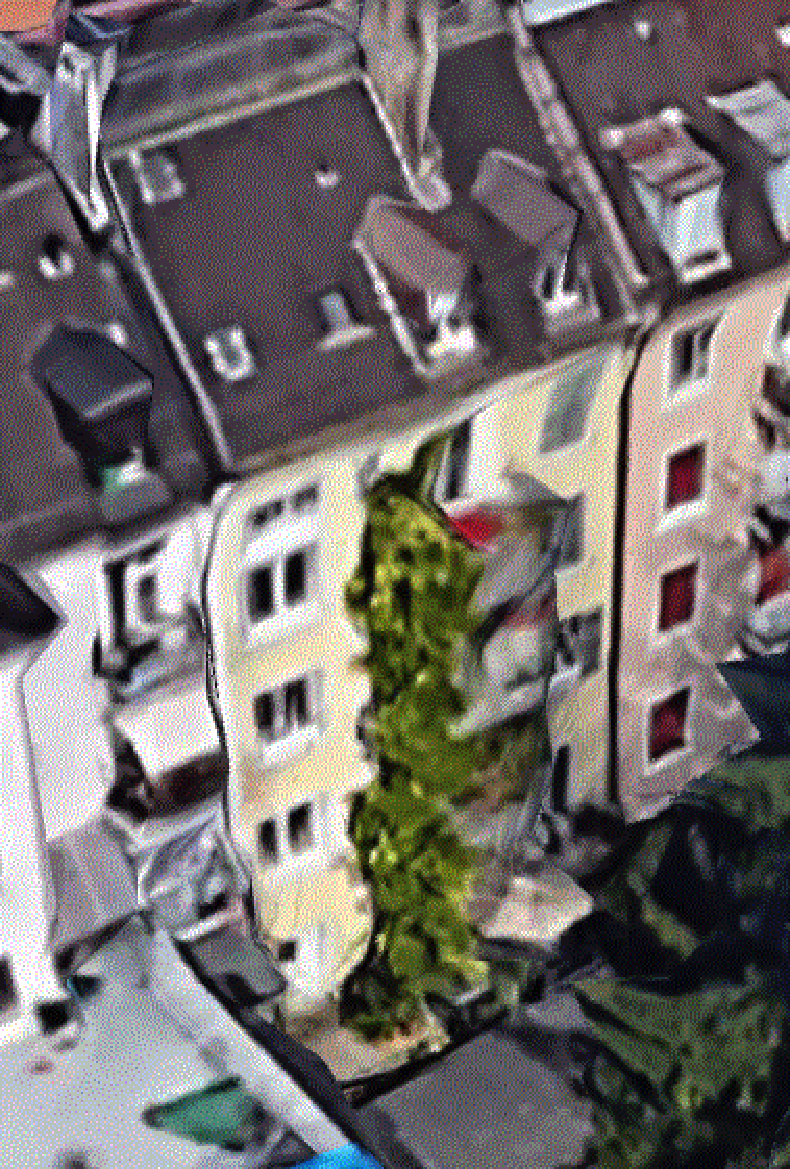
\includegraphics[width=6cm]{Hongg_photo0.pdf}
		\caption{Honggerstrasse 23, SW side}
		\label{fig:hongg_SW}
		\end{minipage}
		\end{figure}

		\begin{figure}[htbp]
		\centering
		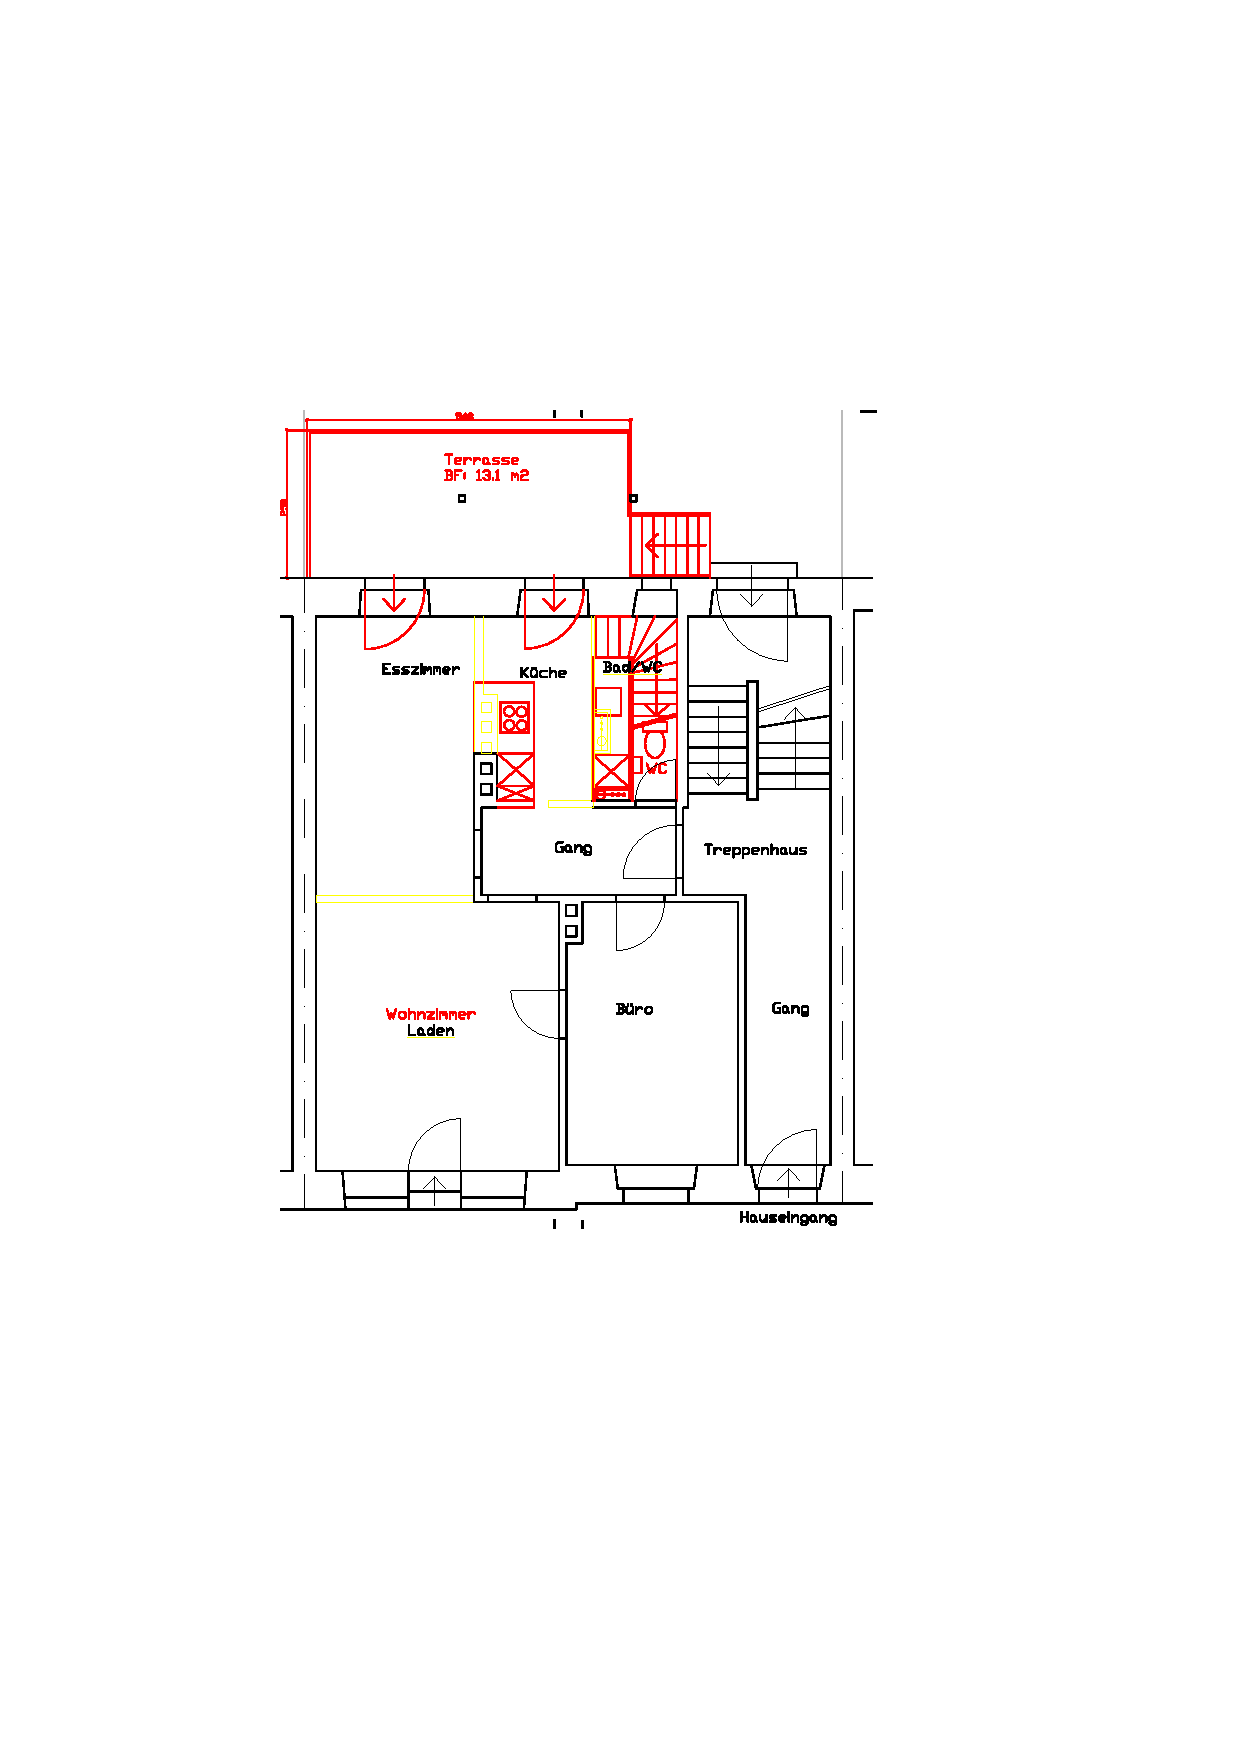
\includegraphics[scale=1.5]{Hongg_EG_Plan.pdf}
		\caption{Floor plan of residential building (Hongger) ground - 1$^{st}$ floor}
		\label{fig:hongg_eg_plan}
		\end{figure}
		
		\begin{figure}[htbp]
		\centering
		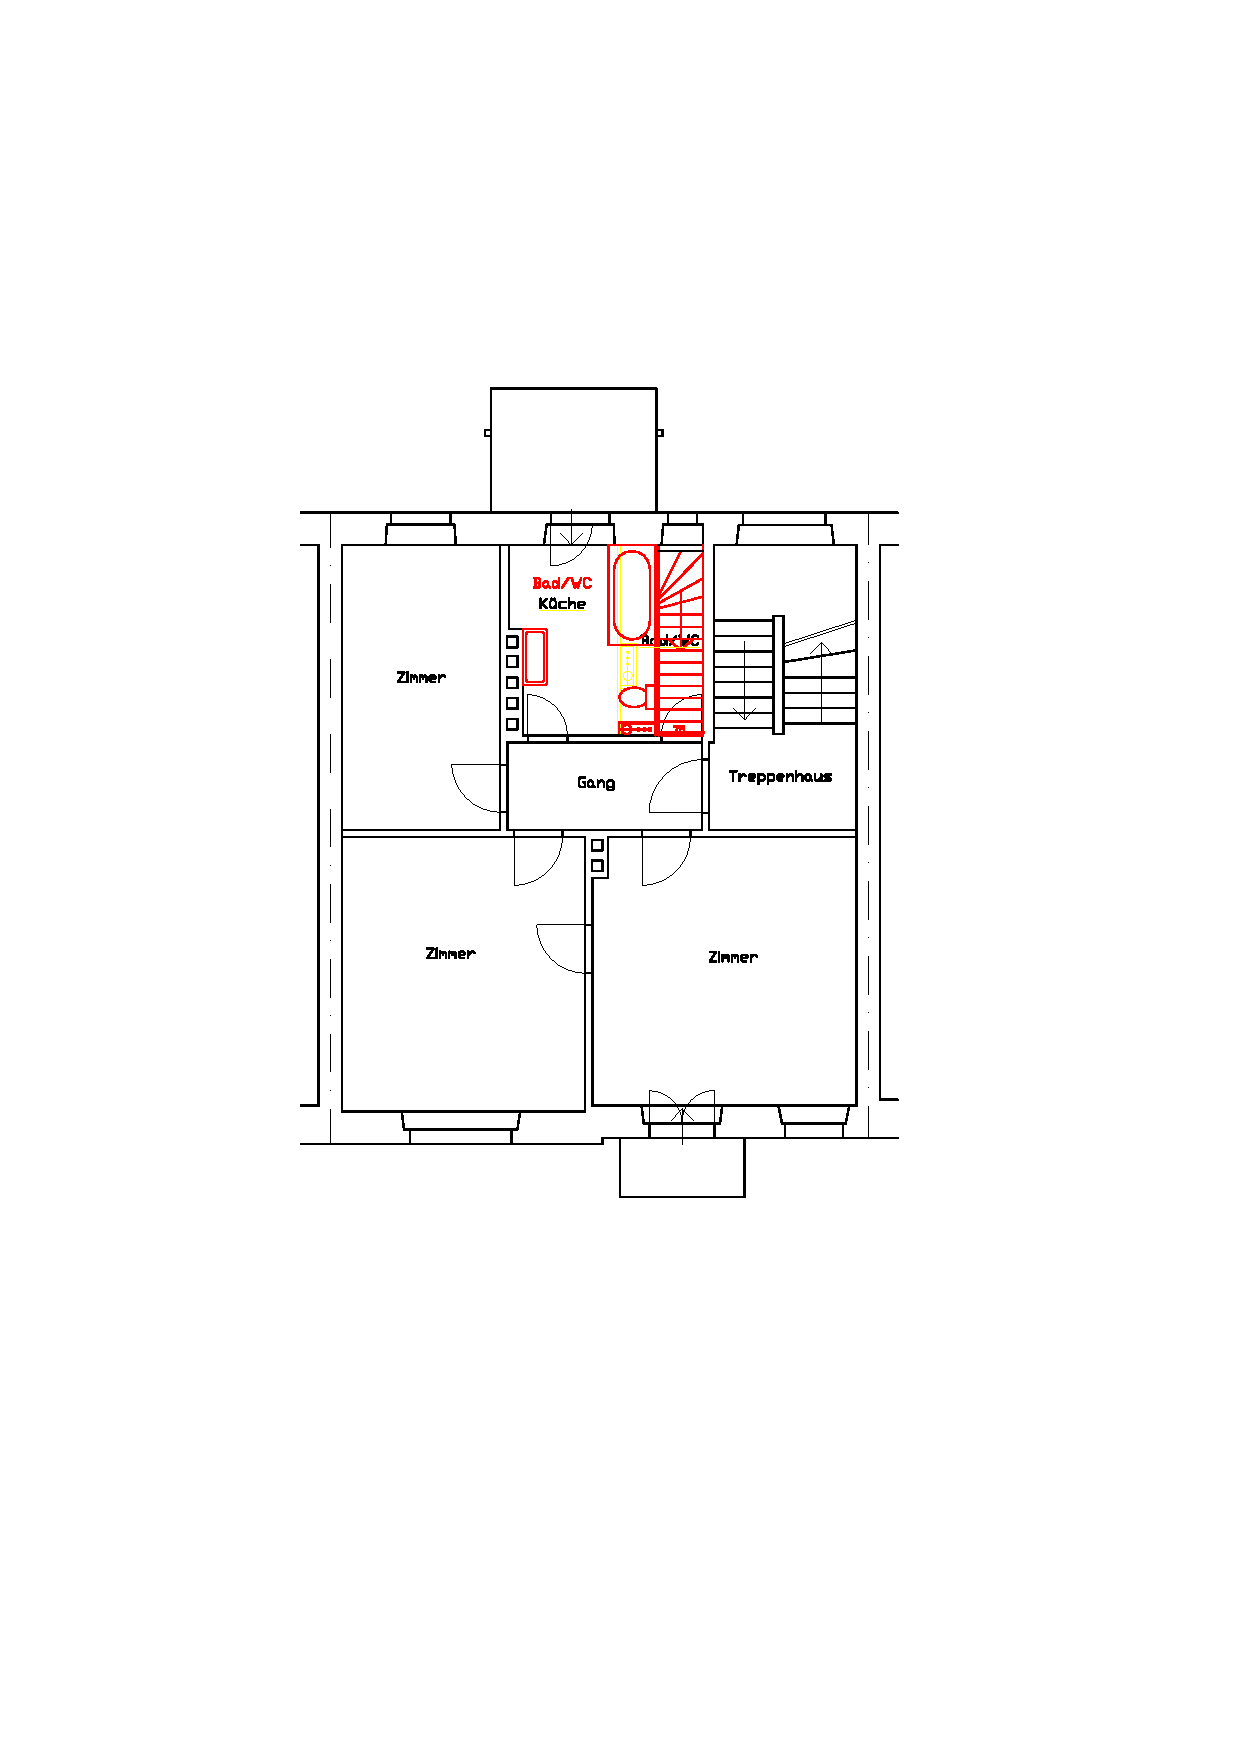
\includegraphics[scale=1.6]{Hongg_1OG_Plan.pdf}
		\caption{Floor plan of residential building (Hongger) 1$^{st} - 4^{th}$ floor}
		\label{fig:hongg_og1_plan}
		\end{figure}


	\section{Building Model Construction}
		\textit{DesignBuilder} is used to model the building envelopes of both buildings. It is compatible with EnergyPlus and provides advanced tools to model building geometry and building system.

		A brief introduction of DesignBuilder, also describe the scope of work (Building envelope, create a formated file for EnergyPlus engine, also provide accurate geometry data for SIA calculation)
		
		\subsection{Building Geometry}
			The actual geometry of the building is not specifically given in the previous report. However, a detailed floor plan and some geometries are given in pdf format as shown above in Figure \ref{fig:sumatra_og2}, and \ref{fig:sumatra_og3}, \ref{fig:hongg_eg_plan}, \ref{fig:hongg_og1_plan}. Therefore, in order to obtain an accurate building geometry, the pdf floor plan is firstly scaled to fit its nominated geometry, then a drawing file with correct scales are made according to the given pdf floor plans. After the drawing files are completed, they can be imported to DesignBuilder as a construction basis as shown in Figure \ref{fig:SumatraDxf} and \ref{fig:HonggerDxf} below.

			\begin{figure}[H]
			\centering
			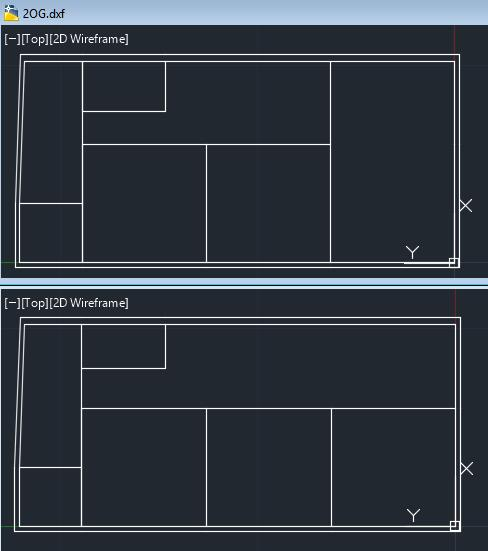
\includegraphics[scale=0.7]{Sumatra_dxf.jpg}
			\caption{dxf drawing files for office building}
			\label{fig:SumatraDxf}
			\end{figure}
			
			\begin{figure}[H]
			\centering
			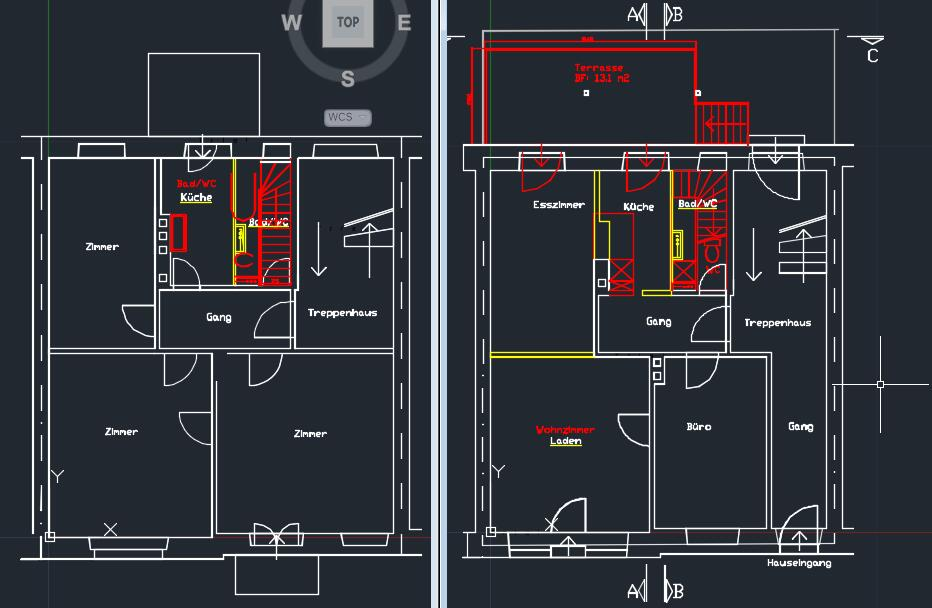
\includegraphics[scale=0.65]{Hongger_dxf.jpg}
			\caption{dxf drawing files for residential building}
			\label{fig:HonggerDxf}
			\end{figure}
			

			After the outline of buildings are constructed, windows and doors are defined. The window and door geometries of the office building and the residential building are shown at the table \ref{table:HonggerWindowLayout} and table \ref{table:SumatraWindowLayout} below. The detailed window code information can be found in Table \ref{tab:SumatraWindow}. \\

				%\newpage
				\begin{table}[H]
				\centering
				\caption{Window Layout of Residential Building}
				\begin{tabular}{  c | c | c | c  }
					\hline
					\multicolumn{4}{c}{Ground Floor} \\ 
					\hline
					Orientation & Location & Window Code & \# of window \\ \hline
					\multirow{4}{*}{SW} & Terrasse & 2a & 2 \\ 
					 & WC & 3a & 1 \\ 
					 & Staircase & 1a & 1 \\ 
					 & Front Door & TH & 1 \\ \hline
					\multirow{3}{*}{NE} & Laden & 1a & 1 \\ 
					 & Office & 4a & 1 \\ 
					 & Door & TH 1a & 1 \\ \hline
					\multicolumn{4}{c}{1st Floor to 4th Floor}\\ \hline
					\multirow{4}{*}{SW} & Terrasse & 2a & 1 \\ 
					 & WC & 3a & 1 \\ 
					 & Office & 4a & 1 \\ 
					 & Corridor & TH 1a & 1 \\ \hline
					\multirow{2}{*}{NE} & Office & 4a & 2 \\ 
					 & Terrasse & 2a & 1 \\ 
					 \hline
				\end{tabular}
				\label{table:HonggerWindowLayout}
				\end{table}


				\begin{table}[H]
				\centering
				\caption{Window Layout of Office Building}
				\begin{tabular}{  c | c | c | c  }
					\hline
					\multicolumn{4}{c}{Ground Floor}\\
					\hline
					Orientation & Location & Code & Number \\ \hline
					\multirow{4}{*}{W} & Right Office & FE1 & 2 \\
					 & Conference room & FE1 & 2 \\
					 & Large office & FE1 & 2 \\
					 & Corridor & FE6 & 2 \\ \hline
					S & Large office & FE6 & 2 \\ \hline
					\multicolumn{4}{c}{1st Floor and 2nd Floor}\\\hline
					\multirow{4}{*}{W} & Right Office & FE1 & 2 \\ 
					 & Conference room & FE1 & 2 \\ 
					 & Large office & FE1 & 2 \\ 
					 & small office & FE1 & 1 \\ \hline
					S & Large office & FE1 & 1 \\ \hline
					\multicolumn{4}{c}{3rd Floor}\\ \hline
					\multirow{4}{*}{W} & Right Office & FE1 & 2 \\ 
					 & Middle office & FE1 & 2 \\ 
					 & Corner office & FE1 & 2 \\ 
					 & small office & FE1 & 1 \\ \hline
					\multirow{3}{*}{S} & Corner office & FE1 & 2 \\ 
					 & Kitchen and Corridor & FE4 & 1 \\ 
					 & Kitchen and Corridor & FE5 & 1 \\ \hline
					\multirow{2}{*}{E} & Kitchen and Corridor & FE7 & 1 \\ 
					 & Staircase & FE3 & 1 \\ \hline
				\end{tabular}
				\label{table:SumatraWindowLayout}
				\end{table}


			
				\begin{table}[H]
				\centering
				\caption{Office building window specification}
			    \begin{tabular}{ccccc}
			    	\toprule
				    \multicolumn{1}{p{3em}}{Code} & \multicolumn{1}{p{3.785em}}{U-Value W/m2K} & \multicolumn{1}{p{4.215em}}{\#} & \multicolumn{1}{p{4.215em}}{unit area} & \multicolumn{1}{p{4em}}{Total Area m$^2$} \\
				    \midrule
				    \multicolumn{1}{c}{FE1} & 2.001 & 33   & 6    & 198 \\
				    \midrule
				    \multicolumn{1}{c}{FE2} & 2.500 & 1    & 8.125 & 8.13 \\
				    \midrule
				    \multicolumn{1}{c}{FE3} & 2.500 & 1    & 2.7  & 2.7 \\
				    \midrule
				    FE4  & 2.048 & 3    & 3.5  & 10.5 \\
				    \midrule
				    FE5  & 2.072 & 3    & 2.598 & 7.79 \\
				    \midrule
				    FE6  & 2.028 & 2    & 2.25 & 4.5 \\
				    \midrule
				    FE7  & 2.042 & 2    & 2.88 & 5.76 \\
				    \midrule
				    FE8  & 1.907 & 3    & 0.975 & 2.93 \\
				    \bottomrule
			    \end{tabular}%
				\label{tab:SumatraWindow}%
				\end{table}%

				% Table generated by Excel2LaTeX from sheet 'HonggerWindows'
				\begin{table}[H]
				\centering
				\caption{Residential building window specification}
				    \begin{tabular}{ccccc}
				    \toprule
				    \multicolumn{1}{p{4.215em}}{Code} & \multicolumn{1}{p{5.145em}}{U-Value W/m2K} & \multicolumn{1}{p{5.145em}}{number of windows} & \multicolumn{1}{p{4.43em}}{unit area} & \multicolumn{1}{p{5.145em}}{Total Area} \\
				    \midrule
				    FE-EG-1a & 2.379 & 1    & 6.9  & 9.9 \\
				    \midrule
				    FE-EG-2a & 2.388 & 10   & 2.6  & 26 \\
				    \midrule
				    FE-EG-3a & 2.19 & 5    & 0.6  & 3 \\
				    \midrule
				    FE-EG-4a & 2.285 & 13   & 1.6  & 20.8 \\
				    \midrule
				    FE-TH-1a & 2.33 & 1    & 2.88 & 3.7 \\
				    \midrule
				    Tur-TH & 3.5  & 1    & 2.5  & 2.5 \\
				    \bottomrule
				    \end{tabular}%
				\label{tab:HonggWindow}%
				\end{table}%


			
		

		\subsection{Building Envelope Material}
			After the building geometry is construct, the building wall and window elements are then assigned a set of thermal properties based on measurememt.
			Both buildings are uninsulated reinforced concrete structure buildings with thin outer and inner plaster layers. The detailed building wall material of both buildings as well as their thermodynamic properties are measured from the actural building and are shown in Table \ref{tab:SumatraWallMaterial} and Table \ref{tab:HonggerWallMat}. The window properties and geometries of both buildings can be found in \ref{tab:SumatraWindow} and \ref{tab:HonggWindow}. Also note that the office building has PV panels on the roof but they are not included in either building geometry or building envelop. After the building material are assigned to all part of the buildings, static calculation and dynamic calculation can be performed.\\

			
			\newpage
			\begin{table}[h!]
			  \centering
			\caption{Wall material list of office building}
			    \begin{tabular}{rrrrrrr}
			    \toprule
			         & \multicolumn{1}{p{4em}}{Thickness \newline{}m} & \multicolumn{1}{p{3.145em}}{Density \newline{}kg/m3} & \multicolumn{1}{p{3.285em}}{Lambda \newline{}W/MK} & \multicolumn{1}{p{3.57em}}{Heat Capacity\newline{} KJ/Kg.K} & \multicolumn{1}{p{2.93em}}{R Value \newline{}m2K/W} & \multicolumn{1}{p{3.145em}}{U Value \newline{}W/m2K} \\
			    \midrule
			    \multicolumn{7}{p{26.86em}}{EG East Wall} \\
			    \multicolumn{1}{l}{Outside convection coefficient} &      &      &      &      &      &  \\
			    \multicolumn{1}{p{6.785em}}{Outer Layer} & 0.36 & 2400 & 2.5  & 1    & 0.144 &  \\
			    \multicolumn{1}{p{6.785em}}{Inner Layer} & 0.01 & 1400 & 0.7  & 1    & 0.014 &  \\
			    \multicolumn{3}{p{13.93em}}{Inside convection coefficientr} &      &      & 0.13 & 7.7 \\
			         &      &      &      &      & 0.288 & 3.4703 \\
			    \midrule
			    \multicolumn{7}{p{26.86em}}{West and Other Wall} \\
			    \multicolumn{4}{p{17.215em}}{Outside convection Coefficient} &      & 0.04 & 25 \\
			    \multicolumn{1}{p{6.785em}}{Outside Layer} & 0.02 & 1400 & 0.7  & 1    & 0.029 & 35 \\
			    \multicolumn{1}{p{6.785em}}{Layer2} & 0.05 & 1100 & 0.44 & 0.94 & 0.114 & 8.8 \\
			    \multicolumn{1}{p{6.785em}}{Middle Layer} & 0.02 & 120  & 0.056 & 1.56 & 0.357 & 2.8 \\
			    \multicolumn{1}{p{6.785em}}{Inside Layer} & 0.15 & 2400 & 2.5  & 1    & 0.06 & 16.667 \\
			    \multicolumn{4}{p{17.215em}}{Inside Convection Coefficient} &      & 0.13 & 7.7 \\
			         &      &      &      &      & 0.729 & 1.3713 \\
			    \midrule
			    \multicolumn{7}{p{26.86em}}{East Wall (Thick)} \\
			    \multicolumn{3}{p{13.93em}}{Outside convection Coefficient} &      &      & 0.04 & 25 \\
			    \multicolumn{1}{p{6.785em}}{Outside Layer} & 0.02 & 1800 & 0.87 & 1    & 0.023 & 43.5 \\
			    \multicolumn{1}{p{6.785em}}{Middle Layer} & 0.36 & 1100 & 0.44 & 0.94 & 0.818 & 1.2222 \\
			    \multicolumn{1}{p{6.785em}}{Inside Layer} & 0.02 & 1400 & 0.7  & 1    & 0.029 & 35 \\
			    \multicolumn{3}{p{13.93em}}{Inside Convection Coefficient} &      &      & 0.13 & 7.7 \\
			         &      &      &      &      & 1.04 & 0.9619 \\
			    \midrule
			    \multicolumn{7}{p{26.86em}}{Ceiling} \\
			    \multicolumn{3}{p{13.93em}}{Outside convection coefficient} &      &      & 0.04 & 25 \\
			    \multicolumn{1}{p{6.785em}}{Layer 1} & 0.04 & 120  & 0.056 & 1.56 & 0.714 &  \\
			    \multicolumn{1}{p{6.785em}}{Layer 2} & 0.0042 & 1100 & 0.23 & 1    & 0.15 &  \\
			    \multicolumn{1}{p{6.785em}}{Layer 3} & 0.0035 & 1100 & 0.23 & 1    & 0.015 &  \\
			    \multicolumn{1}{p{6.785em}}{Layer 4} & 0.001 & 980  & 0.5  & 1.8  & 0.002 &  \\
			    \multicolumn{1}{p{6.785em}}{Layer 5} & 0.22 & 2400 & 2.5  & 1    & 0.088 &  \\
			    \multicolumn{3}{p{13.93em}}{Inside convection coefficientr} &      &      & 0.13 & 7.7 \\
			         &      &      &      &      & 1.139 & 0.8777 \\
			    \midrule
			    \multicolumn{7}{p{26.86em}}{Ground} \\
			    \multicolumn{3}{p{13.93em}}{Outside convection coefficient} &      &      & 0.13 & 7.7 \\
			    \multicolumn{1}{p{6.785em}}{Layer 1} & 0.01 & 120  & 0.056 & 1.56 & 0.179 &  \\
			    \multicolumn{1}{p{6.785em}}{Layer 2} & 0.22 & 2400 & 2.5  & 1    & 0.088 &  \\
			    \multicolumn{3}{p{13.93em}}{Inside convection coefficientr} &      &      & 0.13 & 7.7 \\
			         &      &      &      &      & 0.526 & 1.9 \\
			    \bottomrule
			    \end{tabular}%
			  \label{tab:SumatraWallMaterial}%
			\end{table}%

			\newpage
			\begin{table}[h!]
			  \centering
			\caption{Residential building wall material}
			    \begin{tabular}{rrrrrrr}
			    \toprule
			         & \multicolumn{1}{p{3.93em}}{Thickness m} & \multicolumn{1}{p{3.07em}}{Density kg/m3} & \multicolumn{1}{p{3.145em}}{Lambda W/MK} & \multicolumn{1}{p{3.57em}}{Heat Capacity KJ/Kg.K} & \multicolumn{1}{p{3.355em}}{R Value m2K/W} & \multicolumn{1}{p{3.355em}}{U Value W/m2K} \\
			    \midrule
			    \multicolumn{7}{c}{External Wall} \\
			    \midrule
			    \multicolumn{1}{l}{Outside convection Coefficient} &      &      &      &      & 0.04 & 25 \\
			    \multicolumn{1}{l}{Outside Layer} & 0.04 & 1800 & 0.87 & 1    & 0.046 & 21.75 \\
			    \multicolumn{1}{l}{Middle Layer} & 0.6  & 1800 & 0.8  & 0.94 & 0.75 & 1.3333 \\
			    \multicolumn{1}{l}{Inside Layer} & 0.02 & 1400 & 0.7  & 1    & 0.0286 & 35 \\
			    \multicolumn{1}{l}{Inside Convection Coefficient} &      &      &      &      & 0.1299 & 7.7 \\
			         &      &      &      &      & 0.9944 & 1.0056 \\
			    \midrule
			    \multicolumn{7}{c}{Ground} \\
			    \midrule
			    \multicolumn{1}{l}{Outside convection coefficient} &      &      &      &      & 0.1299 & 7.7 \\
			    \multicolumn{1}{l}{Layer 1} & 0.02 & 900  & 0.25 & 1    & 0.08 &  \\
			    \multicolumn{1}{l}{Layer 2} & 0.1  &      &      &      & 0.15 &  \\
			    \multicolumn{1}{l}{Layer 3} & 0.03 & 1500 & 1.5  & 2.1  & 0.02 &  \\
			    \multicolumn{1}{l}{Layer 4} & 0.03 & 500  & 0.13 & 1.6  & 0.2308 &  \\
			    \multicolumn{1}{l}{Inside convection coefficientr} &      &      &      &      & 0.1299 & 7.7 \\
			         &      &      &      &      & 0.7405 & 1.3504 \\
			    \midrule
			    \multicolumn{7}{c}{Ceiling} \\
			    \midrule
			    \multicolumn{1}{l}{Outside convection coefficient} &      &      &      &      & 0.1299 & 7.7 \\
			    \multicolumn{1}{l}{Layer 1} & 0.02 & 1400 & 0.7  & 1    & 0.0286 &  \\
			    \multicolumn{1}{l}{Layer 2} & 0.2  & 2300 & 2.3  & 1    & 0.087 &  \\
			    \multicolumn{1}{l}{Layer 3} & 0.02 & 1500 & 1.5  & 2.1  & 0.0133 &  \\
			    \multicolumn{1}{l}{Layer 4} & 0.03 & 500  & 0.13 & 1.6  & 0.2308 &  \\
			    \multicolumn{1}{l}{Inside convection coefficientr} &      &      &      &      & 0.1299 & 7.7 \\
			         &      &      &      &      & 0.6194 & 1.6145 \\
			    \bottomrule
			    \end{tabular}%
			  \label{tab:HonggerWallMat}%
			\end{table}%

		Figure \ref{fig:SumatraDB} and \ref{fig:HonggDB} below shows a completed office and residential building DesignBuilder model with geometry and material information.\\

			%\newpage
			\begin{figure}[H]
			\centering
			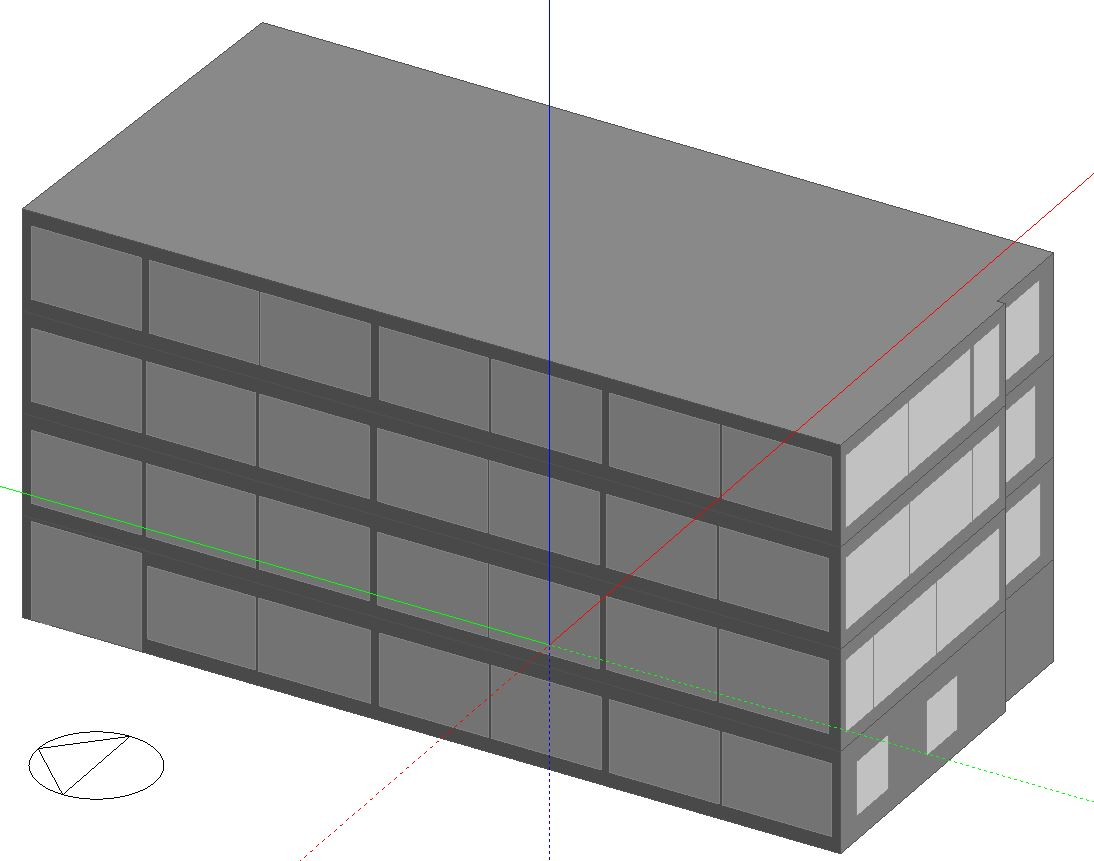
\includegraphics[scale=0.45]{SumatraDesignBuilderModel.JPG}
			\caption{Office building DesignBuilder model}
			\label{fig:SumatraDB}
			\end{figure}

			\begin{figure}[H]
			\centering
			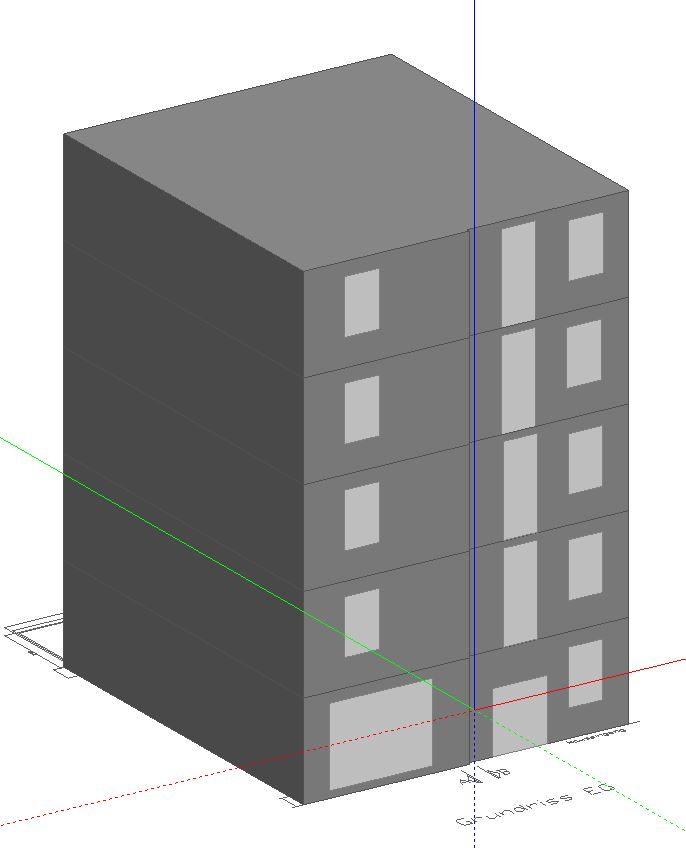
\includegraphics[scale=0.45]{HonggDesignBuilderModel.JPG}
			\caption{Residential building DesignBuilder model}
			\label{fig:HonggDB}
			\end{figure}

			\section{SIA Documentations}
		Most of the building occupancy and activity assumption are from the standard values published by the Swiss society of engineers and architects (hereinafter: SIA Standard). The SIA standards range from energy consumption calculation formulars to the supporting informations about a perticular building type or a room type. It also include a reference standard weather data set for most of the cities in Switzerland. Here are the main SIA standards that are used or taken into account in this thesis.\\

		\textbf{SIA 380/1: Thermal energy in buildings}\\
			This SIA standard is published in 2009 replacing its predecessor SIA 380/1 (2007). It is often used with other standardized calculation parameters when assessing the energy efficiency of existing buildings \cite{SIAPreviousreport}. It also serves as a forecasting tool to evaluate the refurbishment plans. However, the building usually consume less energy than what the calculation suggest, and this issue become more severe as the building envelope gets worse as hown in figure \ref{fig:SIA380PG} below. When using SIA 380/1 to calculate the entitlements for governmental energy certificates, standardized data is used, when using SIA 380/1 for energy consulting, design and optimizations, the best known data is used \cite{SIAPreviousreport}.\\




		\textbf{SIA 2028: SIA Weather Data}\\
			SIA also published a set of standard weather information for most cities in Switzerland. It separates Switzerland into several climate zones and each zone would have their specific climate patten and typical weather data for energy calculation. As SIA 380/1 use monthly average temperature and monthly heating degree days to calculate annual heating demand, this SIA standard weather data is used in this thesis as a reference guide.\\

			The weather data set include monthly and annual average temperature, monthly and annual heating degree days, monthly and annual solar radiation in north, south, east, west and horizontal surfaces. In addition, SIA also published another set of standard hourly data on its partner website \textit{www.energytool.ch} for purchase.\\

		\textbf{SIA 2024: SIA Occupancy and schedule}\\
			Apart from the standard calculation of SIA 380/1 which use monthly and annual unit area standard values for a specific building type, SIA also developed a dynamic building energy analysis approach which use hourly unit area data for a specific room or zone type. SIA 2024 is the unification of assumptions about occupancy and equipment or appliance usage level for specific zone types such as corridor, bedroom, living room and toilet.\\

			The assumptions listed in SIA 2024 include room heating and/or cooling setpoint, maximum supply wind speed, typical room area, window-to-wall ratio, window g-values, room occupancy level and activity level, internal gain level, electricity usage level and activities, minimum and typical amount of outdoor air and ventilation level, lighting and domestic hot water demand etc.\\

			These assumptions are used in calculations and verifications according to energy and building service standard. For occupancy and appliance level assumptions, it gives not only a specific value but also a resonable range which enable a stochastic building energy consumption analysis. SIA 2024 has provide assumptions for 46 different zone types, which cover a majority of building types \cite{SIA2024Shop}.




	


	\newpage

		\section{Weather Data Selection}
			A number of data files or weather data are used during this research. These weather files and data include a typical SIA standard monthly weather and hourly weather; a typical hourly weather file which contains an average or typical weather information from the recent 10 to 15 years; a created data file based on weather station measurement in 2015, and a created heat island weather file. These weather data can be grouped into two categories according to their functions.

			\subsection{Weather Data For Static Calculation}
			\textbf{SIA 381/2 Weather Data}\\
				SIA has published a standard weather data \textit{SIA 381/2 Klimadaten zi Emfehlung SIA 380/1} (Recommended climate data for SOA 380/1) in 1988. It separate Switzerland into a number of climate zones. It also contain monthly weather data set for most main cities in Switzerland. The useful information from this weather dataset are monthly air temperature, monthly heating days, monthly heating degree days and monthly solar radiation on different orientation surfaces.\\


				\begin{table}[H]
				  \centering
				  \small
				\caption{SIA 381/2 Weather Data}
				    \begin{tabular}{|p{5.355em}|c|c|c|c|c|c|c|c|c|c|c|c|c|}
				    \toprule
				    \multicolumn{14}{|c|}{SIA 381/2 Weather Data} \\
				    \midrule
				    \textbf{Month} & \textbf{Jan} & \textbf{Feb} & \textbf{Mar} & \textbf{Apr} & \textbf{May} & \textbf{Jun} & \textbf{Jul} & \textbf{Aug} & \textbf{Sep} & \textbf{Oct} & \textbf{Nov} & \textbf{Dec} & \textbf{Sum} \\
				    \midrule
				    Average Temperature & 0.1  & 2.1  & 4.8  & 9    & 14   & 18   & 19   & 18   & 16   & 11   & 5.4  & 0.6  & 3260 \\
				    \midrule
				    HDD  & 615  & 501  & 467  & 255  & 110  & 23   & 7    & 6    & 35   & 207  & 433  & 601  & 1091 \\
				    \midrule
				    Solar Energy at N (MJ/m2) & 33   & 48   & 78   & 108  & 158  & 172  & 168  & 116  & 89   & 61   & 32   & 28   & 2248 \\
				    \midrule
				    Solar Energy at E (MJ/m2) & 57   & 96   & 170  & 243  & 299  & 320  & 330  & 284  & 212  & 127  & 61   & 49   & 3133 \\
				    \midrule
				    Solar Energy at S (MJ/m2) & 149  & 217  & 281  & 315  & 299  & 290  & 318  & 337  & 347  & 272  & 166  & 142  & 2303 \\
				    \midrule
				    Solar Energy at W (MJ/m2) & 67   & 110  & 170  & 248  & 294  & 308  & 330  & 284  & 227  & 138  & 70   & 57   & 4156 \\
				    \midrule
				    Horizontal Solar Energy & 94   & 166  & 299  & 450  & 565  & 616  & 648  & 526  & 385  & 227  & 104  & 76   & 1564 \\
				    \midrule
				    Solar Energy at NE & 43   & 68   & 115  & 162  & 217  & 235  & 235  & 182  & 137  & 88   & 44   & 37   & 2653 \\
				    \midrule
				    Solar Energy at SW & 100  & 154  & 219  & 279  & 296  & 299  & 324  & 309  & 281  & 194  & 108  & 90   & 2653 \\
				    \bottomrule
				    \end{tabular}%
				  \label{tab:WeatherSIA3812}%
				\end{table}%



			\textbf{2015 Weather Data}\\
				The 2015 Zurich weather data for static calculation is based on the information from the given 2015 .\textit{epw} weather file. The hourly data is firstly extracted from the weather file then calculate the monthly average. \textit{Rhino6} and \textit{Grasshopper} are also used to extract the hourly data as well as calculating the average monthly solar radiation on the nominal orientations (N, E, S, W, NE, SW, and Horizontal). The resultant monthly weather data is shown at Table \ref{tab:2015Monthly}. Table \ref{tab:StaticWeatherCompare} below indicate a comparison of two different weather data.
				
				\begin{table}[H]
				  \centering
				  \small
				\caption{2015 Zurich Monthly Data}
				    \begin{tabular}{|p{5.3em}|r|r|r|r|r|r|r|r|r|r|r|r|r|}
				    \toprule
				    \multicolumn{14}{|c|}{2015 Weather Data} \\
				    \midrule
				    \textbf{Month} & \multicolumn{1}{l|}{\textbf{Jan}} & \multicolumn{1}{l|}{\textbf{Feb}} & \multicolumn{1}{l|}{\textbf{Mar}} & \multicolumn{1}{l|}{\textbf{Apr}} & \multicolumn{1}{l|}{\textbf{May}} & \multicolumn{1}{l|}{\textbf{Jun}} & \multicolumn{1}{l|}{\textbf{Jul}} & \multicolumn{1}{l|}{\textbf{Aug}} & \multicolumn{1}{l|}{\textbf{Sep}} & \multicolumn{1}{l|}{\textbf{Oct}} & \multicolumn{1}{l|}{\textbf{Nov}} & \multicolumn{1}{l|}{\textbf{Dec}} & \multicolumn{1}{l|}{\textbf{Sum}} \\
				    \midrule
				    Average Temperature  & 3.7  & 1.5  & 8.2  & 12   & 16   & 20   & 25   & 23   & 15   & 11   & 9    & 5.1  &  \\
				    \midrule
				    Heating Degree Days & 498  & 519  & 344  & 149  & 31   & 0    & 0    & 0    & 18   & 225  & 268  & 462  & 2513.1 \\
				    \midrule
				    Solar Energy at N (MJ/m2) & 25   & 42   & 62   & 86   & 116  & 158  & 150  & 107  & 74   & 46   & 30   & 23   & 919.15 \\
				    \midrule
				    Solar Energy at E (MJ/m2) & 55   & 103  & 176  & 238  & 289  & 301  & 332  & 278  & 185  & 113  & 65   & 41   & 2176.1 \\
				    \midrule
				    Solar Energy at S (MJ/m2) & 183  & 213  & 304  & 298  & 244  & 237  & 245  & 284  & 279  & 238  & 146  & 116  & 2786.3 \\
				    \midrule
				    Solar Energy at W (MJ/m2) & 67   & 97   & 186  & 233  & 261  & 294  & 299  & 258  & 206  & 127  & 61   & 52   & 2140.7 \\
				    \midrule
				    Horizontal Solar Energy & 104  & 174  & 316  & 446  & 549  & 596  & 605  & 512  & 353  & 208  & 108  & 78   & 4049.9 \\
				    \midrule
				    Solar Energy at NE & 26   & 51   & 92   & 140  & 202  & 231  & 244  & 179  & 108  & 58   & 33   & 24   & 1388.6 \\
				    \midrule
				    Solar Energy at SW & 146  & 167  & 269  & 287  & 273  & 282  & 288  & 290  & 268  & 204  & 112  & 97   & 2683.8 \\
				    \bottomrule
				    \end{tabular}%
				  \label{tab:2015Monthly}%
				\end{table}%

				% Table generated by Excel2LaTeX from sheet 'Sheet2'
				\begin{table}[htbp]
				  \centering
				\caption{Weather Data Comparison}
				    \begin{tabular}{|c|c|c|c|}
				    \toprule
				         & \multicolumn{1}{c}{SIA Standard Weather} & 2015 Weather & Typical Zurich Weather\\
				    \midrule
				    Heating Day & 208  & 175 & 213\\
				    \midrule
				    Heating Degree Day & 3260 & 2513 & 3283\\
				    \midrule
				    Annual Average Temperature & 8.5  & 12.3 & 9.75\\
				    \bottomrule
				    \end{tabular}%
				  \label{tab:StaticWeatherCompare}%
				\end{table}%


			\subsection{Weather Data For Dynamic Calculation}
				An .\textit{epw} weather file is needed for dynamic calculation using \textit{EnergyPlus}. The weather file is either from a meteological organization or from modifying an existing weather file. It contains a large number of weather information such as dry-bulb temperature, wet-bulb temperature, relative humidity, wind speed, wind direction, hourly solar radiation, cloudiness etc.\\

			\textbf{Typical Year Weather File}\\
				A typical year Zurich weather file is given by EMPA research unit. It also become the basis for other custom-made weather files that are used in this thesis. The basic statistic information of the typical year weather file is shown at the 3$^{rd}$ column of Table \ref{tab:StaticWeatherCompare}. \\

			\textbf{2015 Weather File}\\
				The 2015 weather file is created from the typical Zurich weather file by replacing the dry bulb temperature, wet bulb temperature, relative humidity, wind speed, and wind direction by the actual hourly measured data in Zurich in 2015. The source of weather data is from \textit{Federal Office of Meteology and Climatology MeteoSwiss}. Considering the location of the two existing building, the weather station is chosen to be \textit{NABZUE}, which located at Zurich city as shown in Figure \ref{fig:NABZUE}.

				\begin{figure}[H]
				\centering
				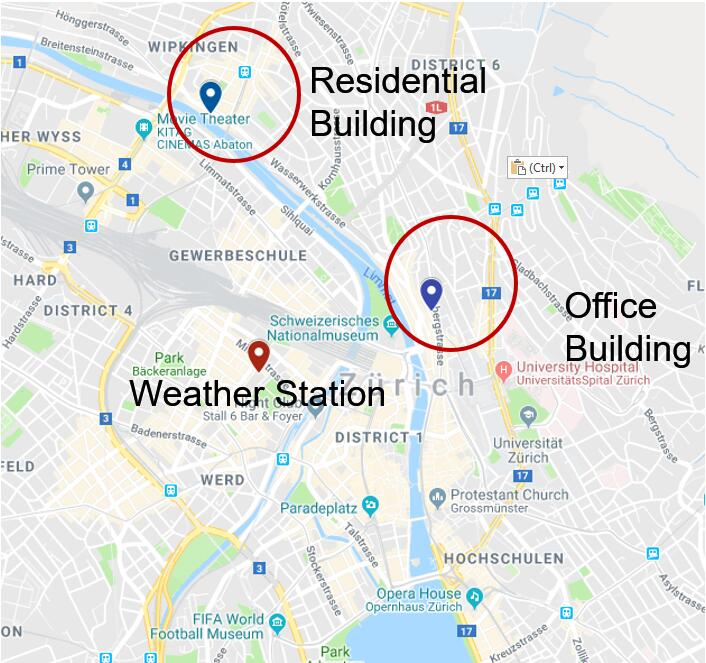
\includegraphics[scale=0.7]{WeatherStation.jpg}
				\caption{Weather Station Location}
				\label{fig:NABZUE}
				\end{figure}
				
				% Table generated by Excel2LaTeX from sheet 'Sheet2'
				\begin{table}[htbp]
				  \centering
				  \caption{Weather Data Information}
				    \begin{tabular}{|c|c|}
				    \toprule
				    \multicolumn{2}{|c|}{\textbf{2015 Weather Data Information}} \\
				    \midrule
				    Source & MeteoSwiss: IDAWEB \\
				    \midrule
				    Weather Station Code & NABZUE \\
				    \midrule
				    Station Coordinate & E 8o31’49” , N 47o22’39” \\
				    \midrule
				    Altitude & 409 m \\
				    \midrule
				    Year & 2015 \\
				    \bottomrule
				    \end{tabular}%
				  \label{tab:2015DataInformation}%
				\end{table}%



			\textbf{SIA382 Weather File}\\
				The full weather data is not fully accessible, and only the hourly temperature is obtained. However, the SIA 382 Weather File is only used to investigate the global warming effect in Zurich. The hourly stand weather temperature is used to replace the typical year weather temperature in the typical year weather file, while all other information remain the same as the 2015 weather data. The comparison between SIA 382 temperature and 2015 actual temperature \\ 

			\textbf{Heat Island Weather File}\\
				Similarly, heat island weather is created based on measured data in year 2015 and aimed to investigate the heat island effect of Zurich city. Firstly, the temperature difference between building site temperature and the weather station data is recorded and average temperature difference is taken hour by hour as shown in Figure \ref{fig:HeatIslandConst} below. Then, a simple rule is apply on the 2015 weather temperature for each hour and create a new heat island weather temperature as shown in Figure \ref{fig:HeatIslandRule}. Lastly, the new heat island temperature is imported to the .\textit{epw} weather file and become the \textit{heat island weather file}.


				\begin{figure}[H]
				\centering
				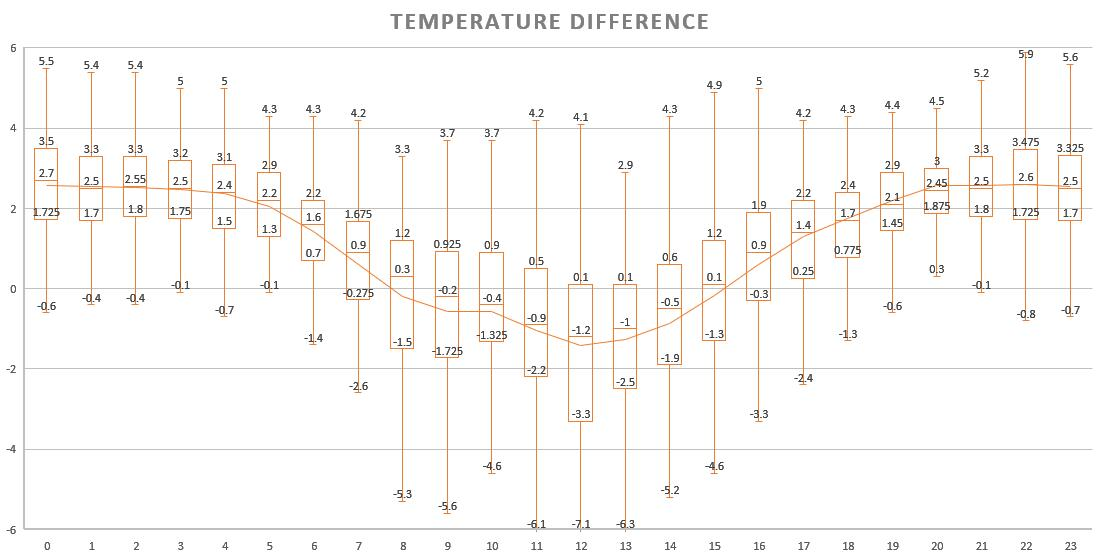
\includegraphics[scale=0.55]{HeatIsland_Construction.jpg}
				\caption{Temperature Difference}
				\label{fig:HeatIslandConst}
				\end{figure}
				
				\begin{figure}[H]
				\centering
				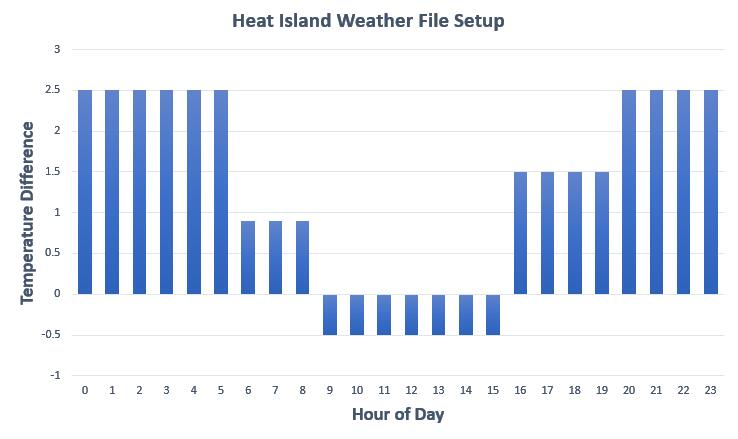
\includegraphics[scale=0.62]{HeatIslandConstruction.jpg}
				\caption{Heat Island Temperature Modification Rule}
				\label{fig:HeatIslandRule}
				\end{figure}
				



	\section{Static Calculation}
		To investigate the cause of huge deviation between previous static calculation and measurement heating demand, a new static calculation is conducted with more accurate geometry and weather information. As static calculation follows the standard method proposed by SIA 180/1. The SIA calculation is divided into several parts. Each part calculates a type of energy loss or energy gain. 

		\subsection{Heat Losses}
			SIA takes a number of losses into account, mainly \textit{transmission loss} and \textit{ventilation loss}. The \textit{transmission loss} includes heat loss through conduction, heat loss through convection, and heat loss through thermal bridge. The losses are calculated based on the building location's heating degree days, building material thermal properties, and the dimension of building elements. The formula for the losses are given below.\\

			\textbf{Transmission Heat Loss}\\

				\[\dot{Q}_{transmission} =\frac{ A_{surface} \cdot U \cdot HDD \cdot 24 \cdot 3600}{A_{floor} \cdot 10^6}\]
				where:\\
				$\dot{Q}_{transmission}$: Heat transmission in $MJ/m^2$\\
				$A_{surface}$: Surface area of building element in $m^2$\\
				$U$: U-Value of building element in $ W/m^2K$\\
				$HDD$: Heating degree days\\
				$A_{floor}$: Total conditioned area of entire building\\

				The ground floor use a different formula to calculate the heat transmission heat loss.
				\[\dot{Q}_{\text{ground}} = \frac{ A_{c} \cdot U \cdot HT \cdot \Delta T \cdot 24 \cdot 3.6}{1000 \cdot A_{floor}}\]
				where:\\
				$A_c$: ground area (in m$^2$)\\
				$HT$: Heating days\\
				$U$: U-value of the element\\
				$\Delta T$: Temperature different between heating setpoint temperature and the unheated zone temperature\\

				The U-value of the building elements can be calculated by the formula below: \\
				\[U = \frac{1}{R_{Ex}+R_{Layer}+R_{In}} = \frac{1}{\frac{1}{h_{ex}}+\sum_{i}\frac{d_i}{\lambda_i} + \frac{1}{h_{in}}}\]
				where:\\
				$h_{ex}$: External heat convection coefficient in $W/m^K$\\
				$h_{in}$: Internal heat convection coefficient\\
				$R_{Layer}$: Total heat resistance of building element in $m^K/W$\\
				$d$: thickness of building element in $m$\\
				$\lambda$: Thermal conductivity of building element in $W/mK$\\


			\textbf{Thermal Bridge Heat Loss}\\
				The loss through thermal bridges can be calculated in the following formula.\\
				\[\dot{Q}_{TB} = \frac{\Psi \cdot L \cdot HDD \cdot 24 \cdot 3600}{A_{floor} \cdot 10^6}\]
				where:\\
				$\dot{Q}_{TB}$: Thermal bridge heat loss in $MJ/m^2$\\
				$L$: Length of thermal bridge\\
				$\Psi$: Thermal bridge loss factor\\ 
				$HDD$: Heating degree days\\
				$A_{floor}$: Total conditioned area of entire building\\


			\textbf{Ventilation Loss}
				The ventilation heat loss is given below:\\
				\[Q_{\text{vent}} = \frac{\dot{V} \cdot c_{p,air} \cdot HDD}{24 \cdot 1000}\]
				where:\\
				$\dot{Q}_{\text{vent}}$: Ventilation heat loss in $MJ/m^2$\\
				$\dot{V} = 0.7$: Ventilation rate in $m^3/m^2\cdot h$\\
				$c_{p,air} = 1.16$: Heat capacity of air $kJ/m^3 \cdot K$\\
				$HDD$: heating degree days\\


		\subsection{Heat Gains}
			In SIA 380/1 calculation, heat gain can be obtained from solar radiations, internal gains by electronics, and internal gains by occupant activities.\\
			
			\textbf{Solar Gains}\\
			The heat gain from solar energy is given below: \\
			\[Q_{\text{solar}} = \frac{G \cdot A_{\text{glazing}} \cdot f_1 \cdot f_2 \cdot f_3 \cdot f_g \cdot g}{A_{floor}} \]

			where:\\
			$f_1$, $f_2$, $f_3$, $f_g$: Reduction factors for shading, frames, overhangs, and impurities on the window, the values are given in previous calculations\\
			$g$: g-value of the window, transmittance\\
			$G$: Unit solar radiation onto the surface in $MJ/m^2$\\
			$A_{\text{glazing}}$: Window area in $m^2$\\

			
			\textbf{Internal Gains by electronics}\\
			The heat gain from electronics comes from a factor of electricity demand.
			\[\dot{Q}_{\text{elec}} = \frac{E_{unit}  \cdot f_{ele} \cdot HT \cdot 3.6}{365} \]
			$\dot{Q}_{\text{elec}}$: Heat gain by electronics in MJ/m$^2$\\
			$E_{unit}$: Unit area electricity demand in $kWh/m^2$\\
			$f_{ele} = 0.7$: electricity gain factor\\
			$HT$: Heating day\\
			$A_{floor}$: Total floor area\\


			\textbf{Internal Gains by person}\\
			The internal gain from occupant activities is given below:\\

			\[Q_{\text{occ}} = \frac{\dot{q}_{pl} \cdot h_{\text{present}} \cdot 365 \cdot 3.6}{\text{Occ} \cdot  1000}\]
			where:\\
			$\dot{Q}_{\text{occ}}$: Internal gains by person in MJ/m$^2$\\
			$\text{Occ}$: Unit area occupancy, Occ = 40$m^2/pl$ for residential, 20$m^2/pl$ for office building\\
			$\dot{q}_{pl} = 70W/pl$: internal gain produce by a single person\\
			$h_{\text{present}}$: present hour per day, 12 for residential building, 6 for office building\\



			\textbf{Total Heat Gain}

			\[Q_{\text{gain}} = (Q_{\text{solar}} + Q_{\text{elec}} + Q_{\text{occ}}) \cdot x\]
			where x is heat gain factor given by:
			\[ x = \frac{\sum \text{Heat Gain}}{\sum \text{Heat Loss}}\]




	
		\subsection{Measurements expected to close the performance gap}
			The building model is firstly subject to static calculation with all standard values and assumptions. After the reference static calculation has been made, another calculation with 2015 weather information is conducted. Depend on the obtained result, further parameters are modified and try to match the calculation results with the measured annual results.

		
	\section{Dynamic Analysis}
		The dynamic analysis include a time-step calculation considering the step change of building thermal information. Therefore, EnergyPlus is used to provide an hourly analysis of the two buildings. A detailed setup of parameters are given below.
		

		
		\subsection{Schedule and Occupancy Assumptions}
			The occupancy schedule and activity level of all zones of the two buildings are from the SIA 2024 standard. The SIA 2024 standard provides a guideline assumptions for different building areas such as bedroom, bathroom, kitchen, office, and corridor.\\

			The detailed information of is stored in separate .\textit{csv} files which contains 8760 entries of hourly data. Below is a list of information obtained from SIA 2024.


				\begin{itemize}
					\item Heating/Cooling Setpoint temperature
					\item Occupancy schedule
					\item Activity level
					\item Lighting Schedule
					\item Lighting Level
					\item Domestic hot water schedule
					\item Domestic hot weater level
					\item Electricity appliance schedule and level
				\end{itemize}
				
			Figure \ref{fig:HeatingSP} below shows the heating setpoints of all zones. Most schedules and activities have a certain weekday/weekend pattern and have different patterns in different months. Figure \ref{fig:JanBathLight} below shows the bathroom lighting schedule in January.\\
			
			\begin{figure}[H]
			\centering
			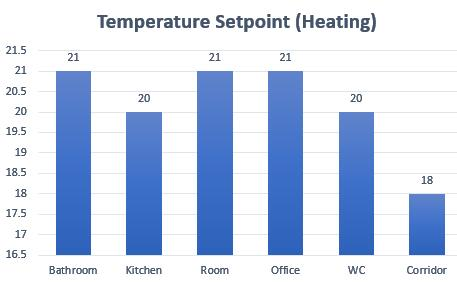
\includegraphics[scale=1]{TempSetpoint.jpg}
			\caption{Heating Temperature Set point}
			\label{fig:HeatingSP}
			\end{figure}
			

			\begin{figure}[h!]
			\centering
			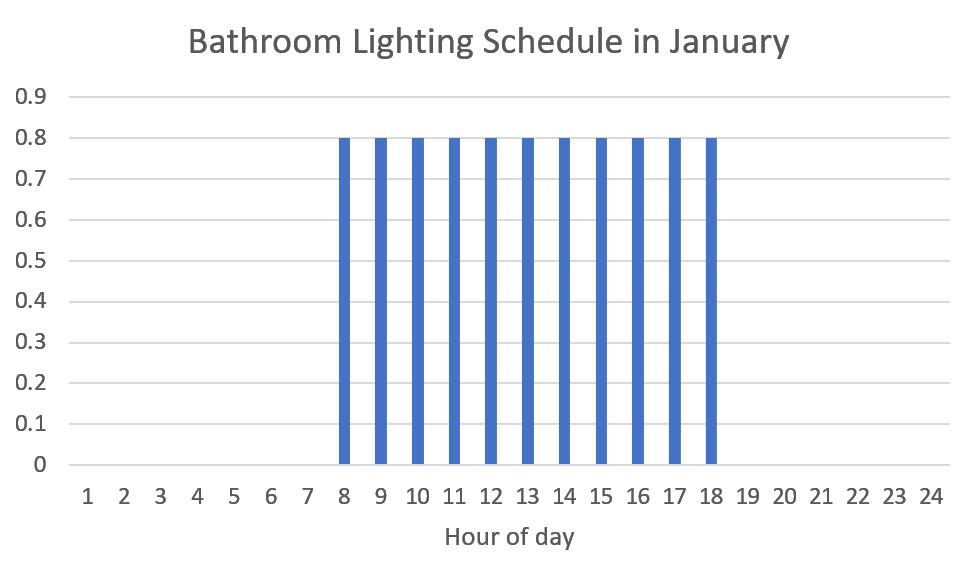
\includegraphics[scale=0.4]{JanBath_Light.jpg}
			\caption{Bathroom Lighting Schedule in January}
			\label{fig:JanBathLight}
			\end{figure}
			



	\section{Calibration}
		In order to ensure the simulated buildings have similar thermal behaviors as the real buildings, a calibration to the building envelope is needed. The calibration process needs to be in a summer period where no heating and cooling is performed. The calibration process vary the building air tightness, internal loads, and user behaviors until the calculated indoor temperature behaves similar enough to the historical measurement. Lastly, the calibrated building is again subject to annual analysis and aim to match the calculated annual energy consumption with the actual measured value.
		

		\subsection{Building Envelope Calibration}
			The air tightness is thought to be an important factor in building simulation. Therefore, the calibration process would vary the air tightness between 0.1 to 0.5 ach and try to match both the hourly indoor temperature as well as the annual heating demand.

		\subsection{Internal Loads}
			Internal load such as Lighting and appliance schedule can change the indoor temperature patten. Therefore, in the calibration process, lighting schedule and electricity schedule are modified to observe the indoor temperature of the focused un-heating period. The newly constructed schedules should be separated into weekday and weekend schedule.

		\subsection{User behavior}
			The user behavior is also thought to be an influential factor to indoor comfort. The calibration also investigate the control strategies for users to operate the window shading. A number of shading control is used and the strategy with most similar indoor temperature patten is used in the calibrated model. The newly constructed shading schedule should vary between summer and winter schedule.


	\section{Parameters Variation}
		After the building model has been constructed and calibrated, a further analysis with varied parameters can be performed. Here are the parameters that are focused and subject to variation:\\
		\begin{itemize}
			\item Heating temperature setpoint for all zones
			\item Occupancy schedule for kay zones (except toilet, wc and corridor)
			\item appliance schedule for all zones (Lighting, Electricity, Domestic hot water)
			\item Ventilation level for all zones
			\item Air infiltration
			\item Internal convection coefficient
			\item External convection coefficient
			\item Facade solar absorptance\\
		\end{itemize}
		
		\textit{jE-Plus}\\
		\textit{jE-Plus} is used as a tool to process the parameter variation analysis. It allows a number of preset parameters to replace certain values in the EnergyPlus file, and allow parallel  There are one thousand building samples with random combination of parameters. \\


		\textit{Heating Temperature Setpoint}\\
			All zones' heating setpoint temperature are part of the parameter variation. The heating setpoint temperature for the same category at the same floor are thought to be identical. For example, the heating setpoint temperature of \textit{Room2} and \textit{Room3} at the second floor would be the same, but might be different to the heating setpoint temperatues for \textit{Room2} and \textit{Room3} at third floor.\\
			The range of temperature setpoints for each zones is shown in Figure \ref{fig:TempSetpoint} below. The temperature setpoint is randomly created in a normal distribution between a pre-set range.\\

			\begin{figure}[H]
			\centering
			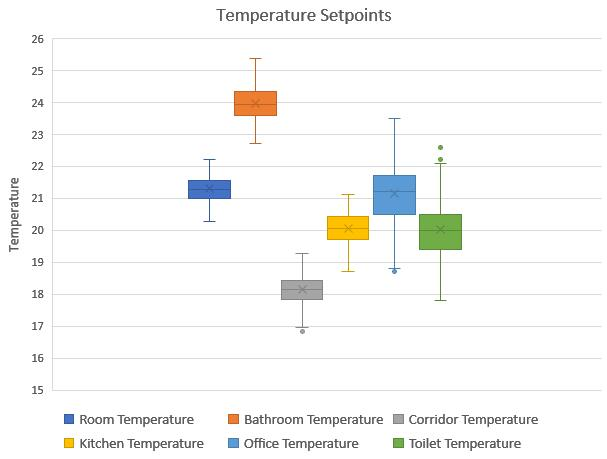
\includegraphics[scale=0.8]{Residential_TempSetpoint.jpg}
			\caption{Heating Temperature Setpoint Distribution}
			\label{fig:TempSetpoint}
			\end{figure}
			
		\textit{Ventilation Level}\\
			Similarly, the ventilation level for each zone is given in Figure \ref{fig:VentLevel} below. The ventilation level for the same zone category at the same floor are thought to be identical. The ventilation level vary according to a normal distribution rule as shown in Figure \ref{fig:VentDist} below.\\
			\begin{figure}[H]
			\centering
			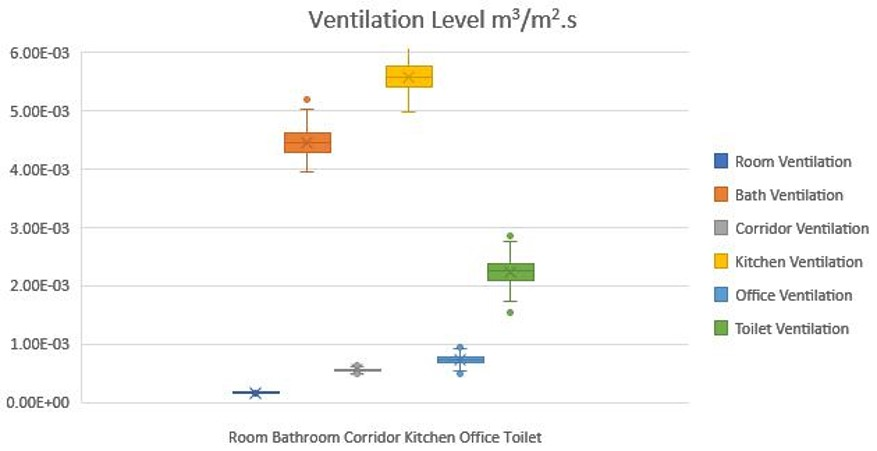
\includegraphics[scale=0.55]{VentilationLevel.jpg}
			\caption{Ventilation Level Distribution}
			\label{fig:VentLevel}
			\end{figure}

			\begin{figure}[H]
			\centering
			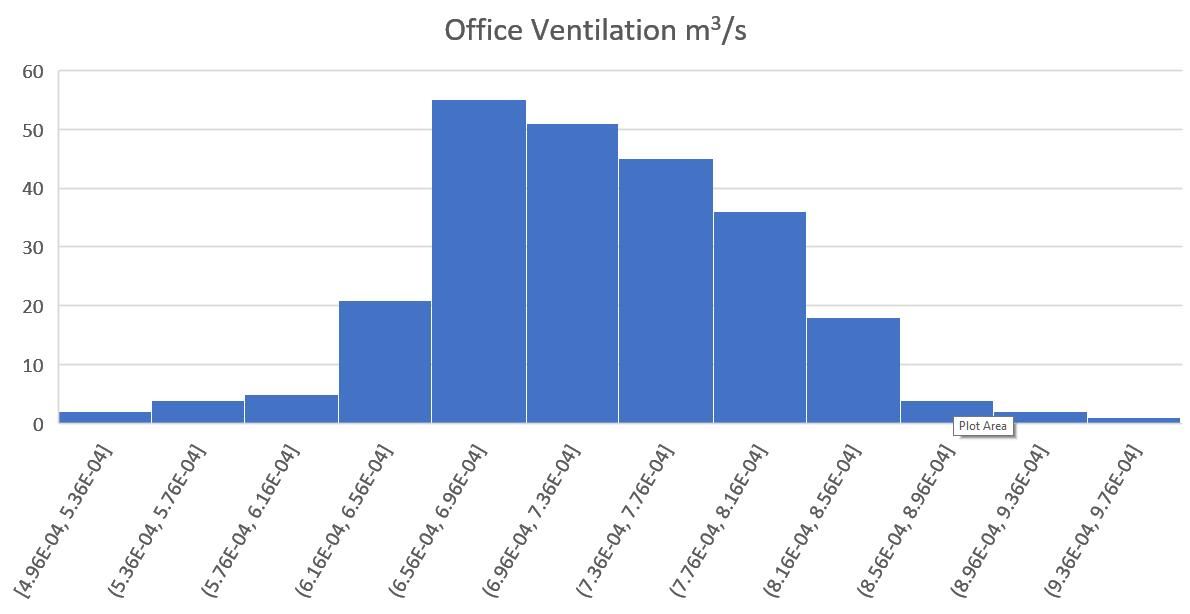
\includegraphics[scale=0.5]{Office_Vent.jpg}
			\caption{Air Ventilation Distribution}
			\label{fig:VentDist}
			\end{figure}
			
			
		\textit{Infiltration}\\
			The infiltration level is roughly a normal distribution which takes $\pm$ 10\% of the calibrated value as its standard deviation. Figure \ref{fig:EXPAirInfiltration_Sumatra} below shows an example air infiltration distribution.\\

			\begin{figure}[H]
			\centering
			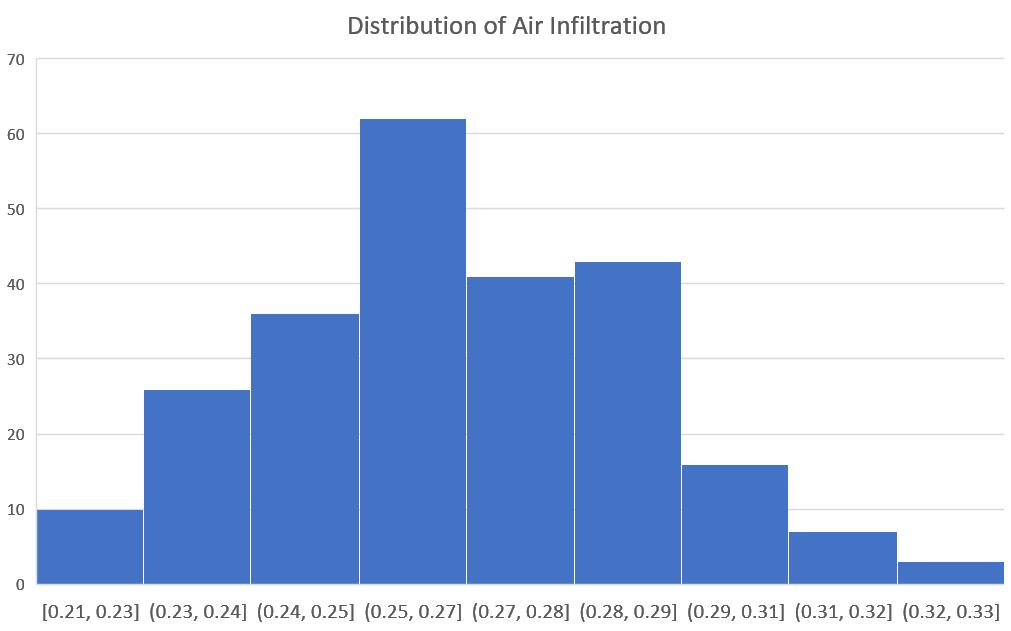
\includegraphics[scale=0.5]{Example_Normal_Distribution.jpg}
			\caption{Example Air Infiltration Distribution}
			\label{fig:EXPAirInfiltration_Sumatra}
			\end{figure}
		
		\textit{Internal and External convection coefficient}\\
			The internal and external convection coefficient range between $\pm 10\%$ of the nominal value.
			A discrete distribution is applied, means the probability of the convection coefficient being any number between $\pm 10\%$ of the nominal value is the same. Figure xx and Figure below shows a distribution histogram of the internal and external heat convection coefficient.\\

			\begin{figure}[H]
			\centering
			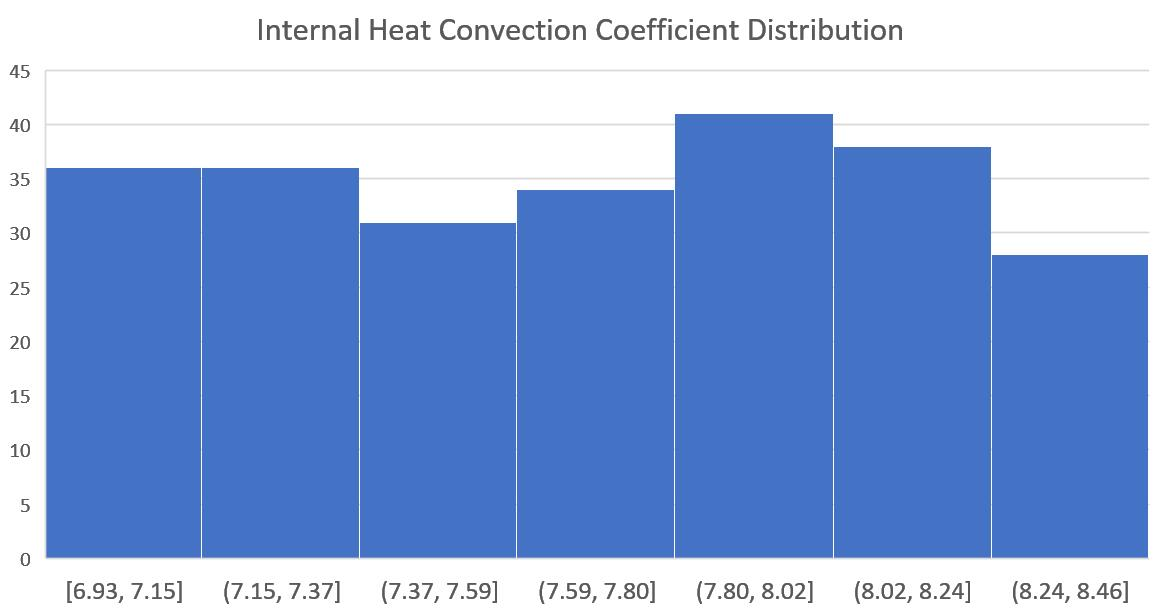
\includegraphics[scale=0.5]{Hongger_InConvDist.jpg}
			\caption{Internal Heat Convection Coefficient Distribution}
			\label{fig:HonggerIntConvDist}
			\end{figure}
			
			\begin{figure}[H]
			\centering
			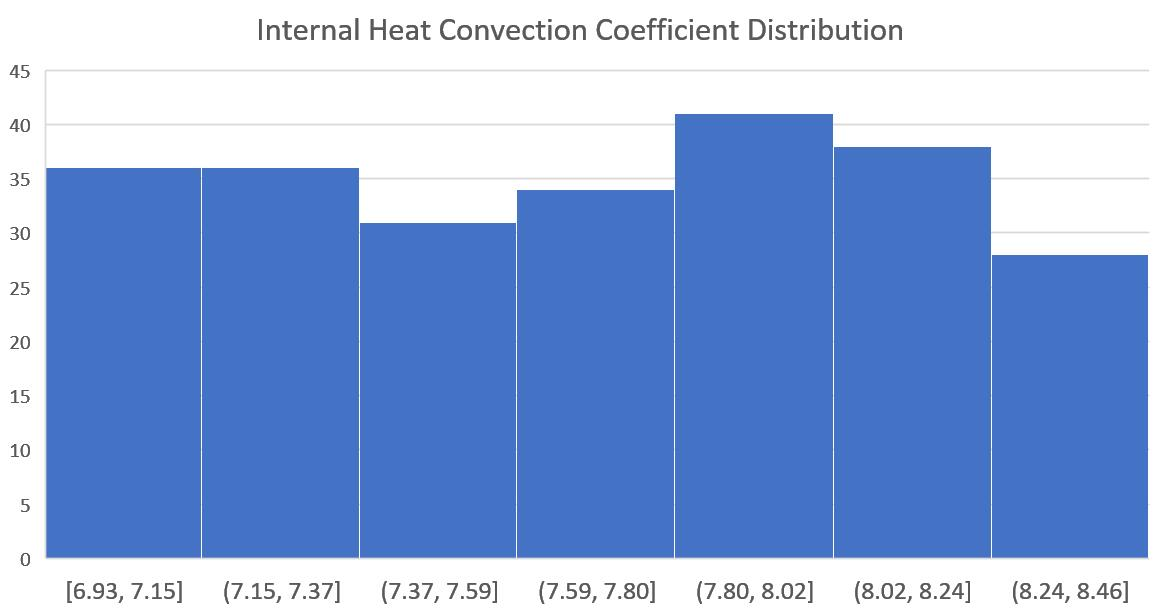
\includegraphics[scale=0.5]{Hongger_InConvDist.jpg}
			\caption{External Heat Convection Coefficient Distribution}
			\label{fig:HonggerExtConvDist}
			\end{figure}
			

		\textit{Facade solar absorptance}\\
			The facade paint and facade color determine the facade solar absorptance. It range from 0 to 1 where a 0 absorptance means the surface reflex all the energy onto the surface, and a 1 absorptance means the facade absorb all the solar energy onto the surface. In this analysis the solar absorptance vary between 0.2 to 0.9 at a discrete distribution.
	
	\section{Data Processing}
		\textit{Python} and Excel are used process the results, where excel is used to generate histograms and other regular charts, while Python (with Matplotlib package) is used to merge data sets, process a series of data files, generate other irregular charts such as correlation matrix, and some boxplots.

		\subsection{Dynamic Analysis Range}
			Histogram and boxplots are used to show the distribution and the range to the dynamic analysis results after the parameter variation. A box is focus on the effect of different simulation environments or parameters while a histogram focus more on the range and the distribution of a single variable.

		\subsection{Correlation Matrix}
			In order to display the relations between parameters and the relations between parameters and heating demands and DHW demands, a correlation matrix is needed to show their influence on each other. \\
			Essentially, the correlation matrix is a heat map matrix where a deeper color represent a higher absolute value. Correlation range between -1 to 1, where -1 and 1 represent a perfect linear relationship and 0 indicates that there is no association between two variables.\\
		



